

%%% outline
%-------------------------------------------------------------------------
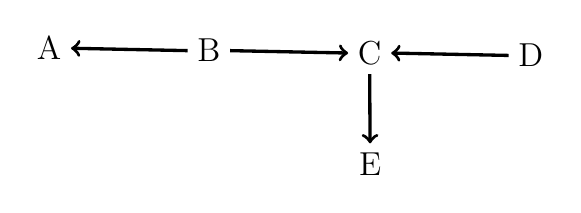
\begin{tikzpicture}


\node [anchor=north west](num1)  at (0,0) {\large{A}};
\node [anchor=north west](num2)  at ([xshift=5.8em,yshift=1.44em]num1.south west) {\large{B}};
\node [anchor=north west](num3)  at ([xshift=5.8em,yshift=1.44em]num2.south west) {\large{C}};
\node [anchor=north west](num4)  at ([xshift=5.8em,yshift=1.44em]num3.south west) {\large{D}};
\node [anchor=north west](num5)  at ([xshift=0.04em,yshift=-2.5em]num3.south west) {\large{E}};


\draw [<-,very thick,black] (num1.east)--(num2.west);
\draw [->,very thick,black] (num2.east)--(num3.west);
\draw [<-,very thick,black] (num3.east)--(num4.west);
\draw [->,very thick,black] (num3.south)--(num5.north);



\end{tikzpicture}
